\documentclass[twoside]{book}

% Packages required by doxygen
\usepackage{fixltx2e}
\usepackage{calc}
\usepackage{doxygen}
\usepackage[export]{adjustbox} % also loads graphicx
\usepackage{graphicx}
\usepackage[utf8]{inputenc}
\usepackage{makeidx}
\usepackage{multicol}
\usepackage{multirow}
\PassOptionsToPackage{warn}{textcomp}
\usepackage{textcomp}
\usepackage[nointegrals]{wasysym}
\usepackage[table]{xcolor}

% Font selection
\usepackage[T1]{fontenc}
\usepackage[scaled=.90]{helvet}
\usepackage{courier}
\usepackage{amssymb}
\usepackage{sectsty}
\renewcommand{\familydefault}{\sfdefault}
\allsectionsfont{%
  \fontseries{bc}\selectfont%
  \color{darkgray}%
}
\renewcommand{\DoxyLabelFont}{%
  \fontseries{bc}\selectfont%
  \color{darkgray}%
}
\newcommand{\+}{\discretionary{\mbox{\scriptsize$\hookleftarrow$}}{}{}}

% Page & text layout
\usepackage{geometry}
\geometry{%
  a4paper,%
  top=2.5cm,%
  bottom=2.5cm,%
  left=2.5cm,%
  right=2.5cm%
}
\tolerance=750
\hfuzz=15pt
\hbadness=750
\setlength{\emergencystretch}{15pt}
\setlength{\parindent}{0cm}
\setlength{\parskip}{0.2cm}
\makeatletter
\renewcommand{\paragraph}{%
  \@startsection{paragraph}{4}{0ex}{-1.0ex}{1.0ex}{%
    \normalfont\normalsize\bfseries\SS@parafont%
  }%
}
\renewcommand{\subparagraph}{%
  \@startsection{subparagraph}{5}{0ex}{-1.0ex}{1.0ex}{%
    \normalfont\normalsize\bfseries\SS@subparafont%
  }%
}
\makeatother

% Headers & footers
\usepackage{fancyhdr}
\pagestyle{fancyplain}
\fancyhead[LE]{\fancyplain{}{\bfseries\thepage}}
\fancyhead[CE]{\fancyplain{}{}}
\fancyhead[RE]{\fancyplain{}{\bfseries\leftmark}}
\fancyhead[LO]{\fancyplain{}{\bfseries\rightmark}}
\fancyhead[CO]{\fancyplain{}{}}
\fancyhead[RO]{\fancyplain{}{\bfseries\thepage}}
\fancyfoot[LE]{\fancyplain{}{}}
\fancyfoot[CE]{\fancyplain{}{}}
\fancyfoot[RE]{\fancyplain{}{\bfseries\scriptsize Generated by Doxygen }}
\fancyfoot[LO]{\fancyplain{}{\bfseries\scriptsize Generated by Doxygen }}
\fancyfoot[CO]{\fancyplain{}{}}
\fancyfoot[RO]{\fancyplain{}{}}
\renewcommand{\footrulewidth}{0.4pt}
\renewcommand{\chaptermark}[1]{%
  \markboth{#1}{}%
}
\renewcommand{\sectionmark}[1]{%
  \markright{\thesection\ #1}%
}

% Indices & bibliography
\usepackage{natbib}
\usepackage[titles]{tocloft}
\setcounter{tocdepth}{3}
\setcounter{secnumdepth}{5}
\makeindex

% Hyperlinks (required, but should be loaded last)
\usepackage{ifpdf}
\ifpdf
  \usepackage[pdftex,pagebackref=true]{hyperref}
\else
  \usepackage[ps2pdf,pagebackref=true]{hyperref}
\fi
\hypersetup{%
  colorlinks=true,%
  linkcolor=blue,%
  citecolor=blue,%
  unicode%
}

% Custom commands
\newcommand{\clearemptydoublepage}{%
  \newpage{\pagestyle{empty}\cleardoublepage}%
}


%===== C O N T E N T S =====

\begin{document}

% Titlepage & ToC
\hypersetup{pageanchor=false,
             bookmarks=true,
             bookmarksnumbered=true,
             pdfencoding=unicode
            }
\pagenumbering{roman}
\begin{titlepage}
\vspace*{7cm}
\begin{center}%
{\Large My Project }\\
\vspace*{1cm}
{\large Generated by Doxygen 1.8.10}\\
\end{center}
\end{titlepage}
\clearemptydoublepage
\tableofcontents
\clearemptydoublepage
\pagenumbering{arabic}
\hypersetup{pageanchor=true}

%--- Begin generated contents ---
\chapter{Hierarchical Index}
\section{Class Hierarchy}
This inheritance list is sorted roughly, but not completely, alphabetically\+:\begin{DoxyCompactList}
\item \contentsline{section}{Distance}{\pageref{classDistance}}{}
\begin{DoxyCompactList}
\item \contentsline{section}{Average\+Distance}{\pageref{classAverageDistance}}{}
\item \contentsline{section}{Euclidian\+Distance}{\pageref{classEuclidianDistance}}{}
\item \contentsline{section}{Max\+Distance}{\pageref{classMaxDistance}}{}
\item \contentsline{section}{Median\+Distance}{\pageref{classMedianDistance}}{}
\end{DoxyCompactList}
\item \contentsline{section}{Distance\+Array}{\pageref{classDistanceArray}}{}
\item \contentsline{section}{Point3\+D}{\pageref{classPoint3D}}{}
\item \contentsline{section}{Pose}{\pageref{classPose}}{}
\item \contentsline{section}{Pose\+Display}{\pageref{classPoseDisplay}}{}
\item \contentsline{section}{Pose\+Sequence}{\pageref{classPoseSequence}}{}
\end{DoxyCompactList}

\chapter{Class Index}
\section{Class List}
Here are the classes, structs, unions and interfaces with brief descriptions\+:\begin{DoxyCompactList}
\item\contentsline{section}{\hyperlink{classAverageDistance}{Average\+Distance} }{\pageref{classAverageDistance}}{}
\item\contentsline{section}{\hyperlink{classDistance}{Distance} }{\pageref{classDistance}}{}
\item\contentsline{section}{\hyperlink{classDistanceArray}{Distance\+Array} }{\pageref{classDistanceArray}}{}
\item\contentsline{section}{\hyperlink{classEuclidianDistance}{Euclidian\+Distance} }{\pageref{classEuclidianDistance}}{}
\item\contentsline{section}{\hyperlink{classMaxDistance}{Max\+Distance} }{\pageref{classMaxDistance}}{}
\item\contentsline{section}{\hyperlink{classMedianDistance}{Median\+Distance} }{\pageref{classMedianDistance}}{}
\item\contentsline{section}{\hyperlink{classPoint3D}{Point3\+D} \\*Real-\/valued points in 3 space, i.\+e. (x, y, z) }{\pageref{classPoint3D}}{}
\item\contentsline{section}{\hyperlink{classPose}{Pose} }{\pageref{classPose}}{}
\item\contentsline{section}{\hyperlink{classPoseDisplay}{Pose\+Display} \\*Class for outputting and (optionally) displaying body poses expressed as a vector of 25 Point3\+Ds }{\pageref{classPoseDisplay}}{}
\item\contentsline{section}{\hyperlink{classPoseSequence}{Pose\+Sequence} }{\pageref{classPoseSequence}}{}
\end{DoxyCompactList}

\chapter{File Index}
\section{File List}
Here is a list of all documented files with brief descriptions\+:\begin{DoxyCompactList}
\item\contentsline{section}{{\bfseries Distance.\+h} }{\pageref{Distance_8h}}{}
\item\contentsline{section}{{\bfseries Distance\+Array.\+h} }{\pageref{DistanceArray_8h}}{}
\item\contentsline{section}{\hyperlink{Point3D_8h}{Point3\+D.\+h} \\*Contains the \hyperlink{classPoint3D}{Point3\+D} class declaration (header) }{\pageref{Point3D_8h}}{}
\item\contentsline{section}{{\bfseries Pose.\+h} }{\pageref{Pose_8h}}{}
\item\contentsline{section}{\hyperlink{PoseDisplay_8cpp}{Pose\+Display.\+cpp} \\*Contains the \hyperlink{classPoseDisplay}{Pose\+Display} class implementation }{\pageref{PoseDisplay_8cpp}}{}
\item\contentsline{section}{\hyperlink{PoseDisplay_8h}{Pose\+Display.\+h} \\*Contains the \hyperlink{classPoseDisplay}{Pose\+Display} class declaration (header) }{\pageref{PoseDisplay_8h}}{}
\item\contentsline{section}{{\bfseries Pose\+Sequence.\+h} }{\pageref{PoseSequence_8h}}{}
\end{DoxyCompactList}

\chapter{Class Documentation}
\hypertarget{classAverageDistance}{}\section{Average\+Distance Class Reference}
\label{classAverageDistance}\index{Average\+Distance@{Average\+Distance}}
Inheritance diagram for Average\+Distance\+:\begin{figure}[H]
\begin{center}
\leavevmode
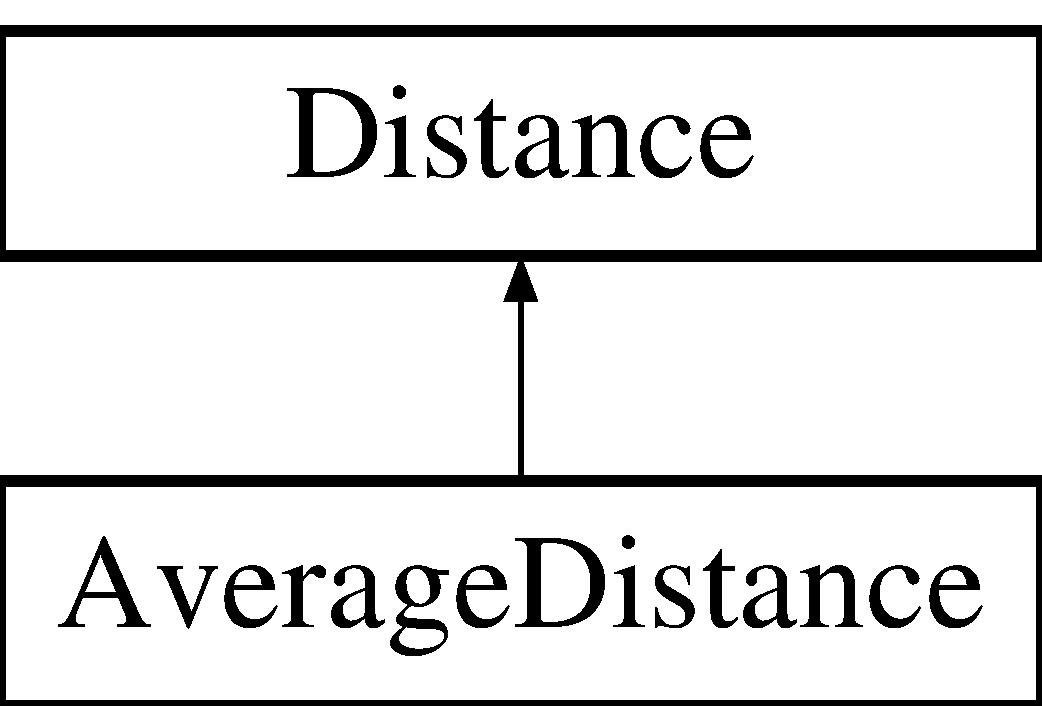
\includegraphics[height=2.000000cm]{classAverageDistance}
\end{center}
\end{figure}
\subsection*{Public Member Functions}
\begin{DoxyCompactItemize}
\item 
\hypertarget{classAverageDistance_a131c831306970b481cb8a35008c73326}{}virtual double {\bfseries pose\+Distance} (const \hyperlink{classPose}{Pose} \&a, const \hyperlink{classPose}{Pose} \&b)\label{classAverageDistance_a131c831306970b481cb8a35008c73326}

\end{DoxyCompactItemize}
\subsection*{Additional Inherited Members}


The documentation for this class was generated from the following files\+:\begin{DoxyCompactItemize}
\item 
Distance.\+h\item 
Distance.\+cpp\end{DoxyCompactItemize}

\hypertarget{classDistance}{}\section{Distance Class Reference}
\label{classDistance}\index{Distance@{Distance}}
Inheritance diagram for Distance\+:\begin{figure}[H]
\begin{center}
\leavevmode
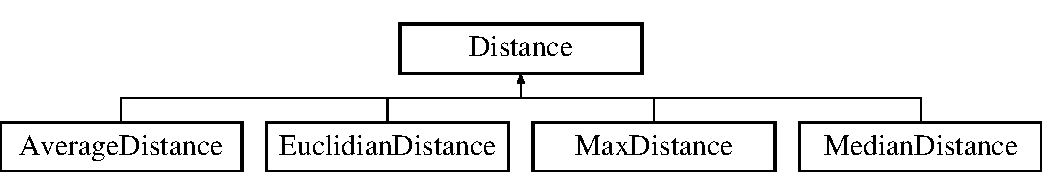
\includegraphics[height=2.000000cm]{classDistance}
\end{center}
\end{figure}
\subsection*{Public Member Functions}
\begin{DoxyCompactItemize}
\item 
\hypertarget{classDistance_a66b5874c975151d95ec87a09d719a0d6}{}virtual double {\bfseries pose\+Distance} (const \hyperlink{classPose}{Pose} \&a, const \hyperlink{classPose}{Pose} \&b)\label{classDistance_a66b5874c975151d95ec87a09d719a0d6}

\end{DoxyCompactItemize}
\subsection*{Static Public Member Functions}
\begin{DoxyCompactItemize}
\item 
\hypertarget{classDistance_a0272fda98bae3f8d8a5c208e61e6b9f6}{}static \hyperlink{classDistance}{Distance} $\ast$ {\bfseries get\+Distance} (const char $\ast$dist\+Type)\label{classDistance_a0272fda98bae3f8d8a5c208e61e6b9f6}

\end{DoxyCompactItemize}


The documentation for this class was generated from the following files\+:\begin{DoxyCompactItemize}
\item 
Distance.\+h\item 
Distance.\+cpp\end{DoxyCompactItemize}

\hypertarget{classDistanceArray}{}\section{Distance\+Array Class Reference}
\label{classDistanceArray}\index{Distance\+Array@{Distance\+Array}}
\subsection*{Public Member Functions}
\begin{DoxyCompactItemize}
\item 
\hypertarget{classDistanceArray_ab84470888c50b602528d99860812404d}{}void {\bfseries pose\+Sequence\+Compare} (const \hyperlink{classPoseSequence}{Pose\+Sequence} \&a, const \hyperlink{classPoseSequence}{Pose\+Sequence} \&b, \hyperlink{classDistance}{Distance} \&d)\label{classDistanceArray_ab84470888c50b602528d99860812404d}

\item 
\hypertarget{classDistanceArray_abfefe1b3d781a062854d6a2191dc1194}{}void {\bfseries print\+Array} () const \label{classDistanceArray_abfefe1b3d781a062854d6a2191dc1194}

\item 
\hypertarget{classDistanceArray_a099459f0426eae862635871c85765b27}{}double {\bfseries dynamic\+Time\+Warping} ()\label{classDistanceArray_a099459f0426eae862635871c85765b27}

\end{DoxyCompactItemize}
\subsection*{Protected Attributes}
\begin{DoxyCompactItemize}
\item 
\hypertarget{classDistanceArray_a924227e33f2574d2bae0f35e9d73bcef}{}vector$<$ vector$<$ double $>$ $>$ {\bfseries distances}\label{classDistanceArray_a924227e33f2574d2bae0f35e9d73bcef}

\end{DoxyCompactItemize}


The documentation for this class was generated from the following files\+:\begin{DoxyCompactItemize}
\item 
Distance\+Array.\+h\item 
Distance\+Array.\+cpp\end{DoxyCompactItemize}

\hypertarget{classEuclidianDistance}{}\section{Euclidian\+Distance Class Reference}
\label{classEuclidianDistance}\index{Euclidian\+Distance@{Euclidian\+Distance}}
Inheritance diagram for Euclidian\+Distance\+:\begin{figure}[H]
\begin{center}
\leavevmode
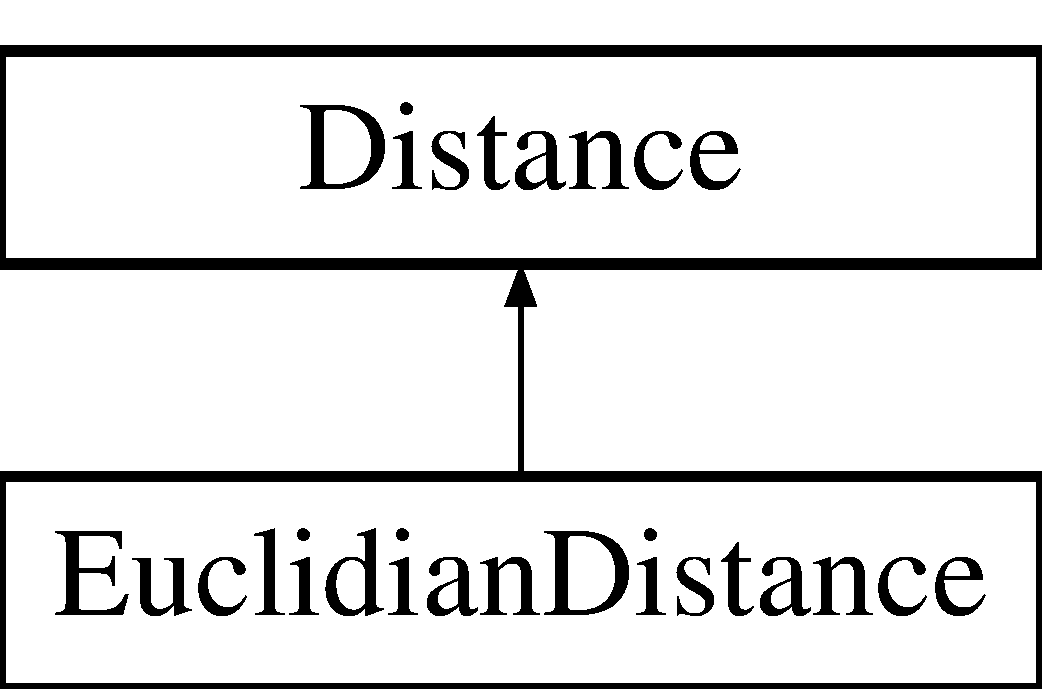
\includegraphics[height=2.000000cm]{classEuclidianDistance}
\end{center}
\end{figure}
\subsection*{Public Member Functions}
\begin{DoxyCompactItemize}
\item 
\hypertarget{classEuclidianDistance_a431698e73e8c884d710c40a9d1541833}{}virtual double {\bfseries pose\+Distance} (const \hyperlink{classPose}{Pose} \&a, const \hyperlink{classPose}{Pose} \&b)\label{classEuclidianDistance_a431698e73e8c884d710c40a9d1541833}

\end{DoxyCompactItemize}
\subsection*{Additional Inherited Members}


The documentation for this class was generated from the following files\+:\begin{DoxyCompactItemize}
\item 
Distance.\+h\item 
Distance.\+cpp\end{DoxyCompactItemize}

\hypertarget{classMaxDistance}{}\section{Max\+Distance Class Reference}
\label{classMaxDistance}\index{Max\+Distance@{Max\+Distance}}
Inheritance diagram for Max\+Distance\+:\begin{figure}[H]
\begin{center}
\leavevmode
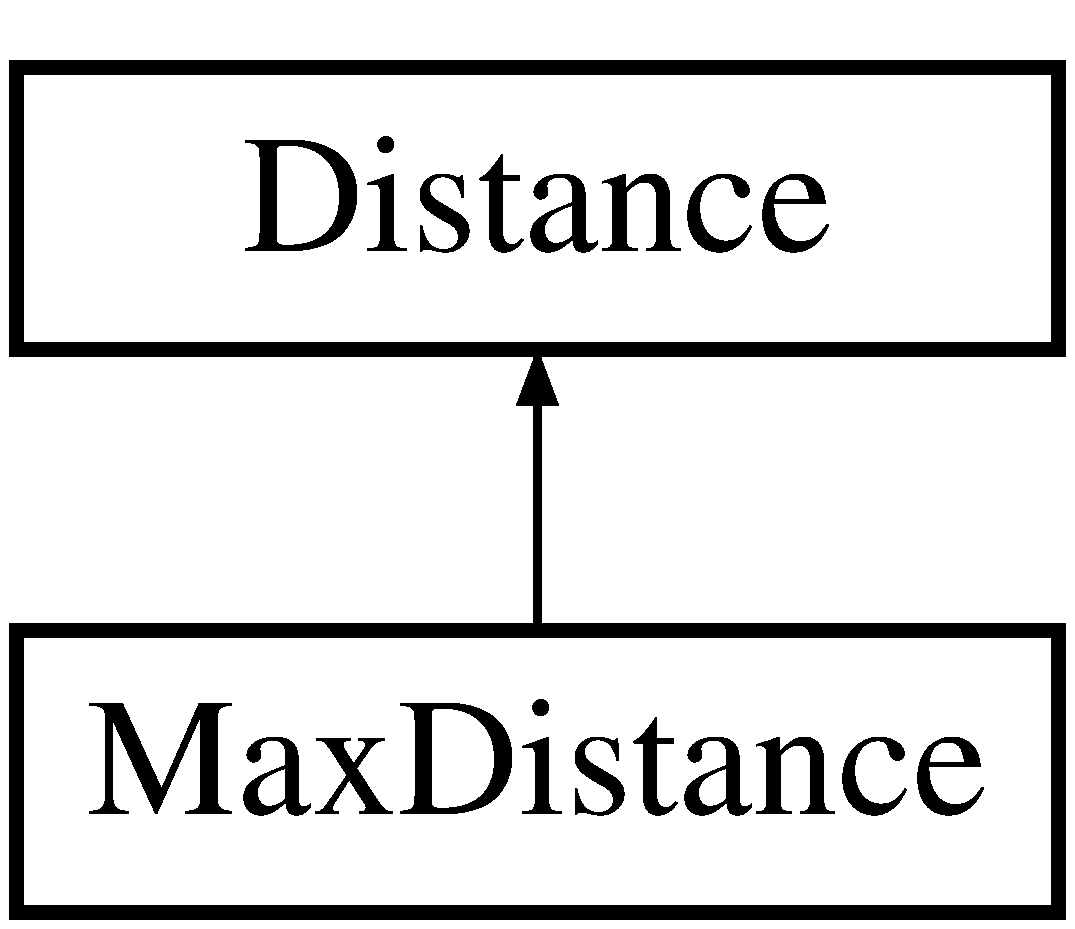
\includegraphics[height=2.000000cm]{classMaxDistance}
\end{center}
\end{figure}
\subsection*{Public Member Functions}
\begin{DoxyCompactItemize}
\item 
\hypertarget{classMaxDistance_a9decef3b40da1568a12c87d4934a9c05}{}virtual double {\bfseries pose\+Distance} (const \hyperlink{classPose}{Pose} \&a, const \hyperlink{classPose}{Pose} \&b)\label{classMaxDistance_a9decef3b40da1568a12c87d4934a9c05}

\end{DoxyCompactItemize}
\subsection*{Additional Inherited Members}


The documentation for this class was generated from the following files\+:\begin{DoxyCompactItemize}
\item 
Distance.\+h\item 
Distance.\+cpp\end{DoxyCompactItemize}

\hypertarget{classMedianDistance}{}\section{Median\+Distance Class Reference}
\label{classMedianDistance}\index{Median\+Distance@{Median\+Distance}}
Inheritance diagram for Median\+Distance\+:\begin{figure}[H]
\begin{center}
\leavevmode
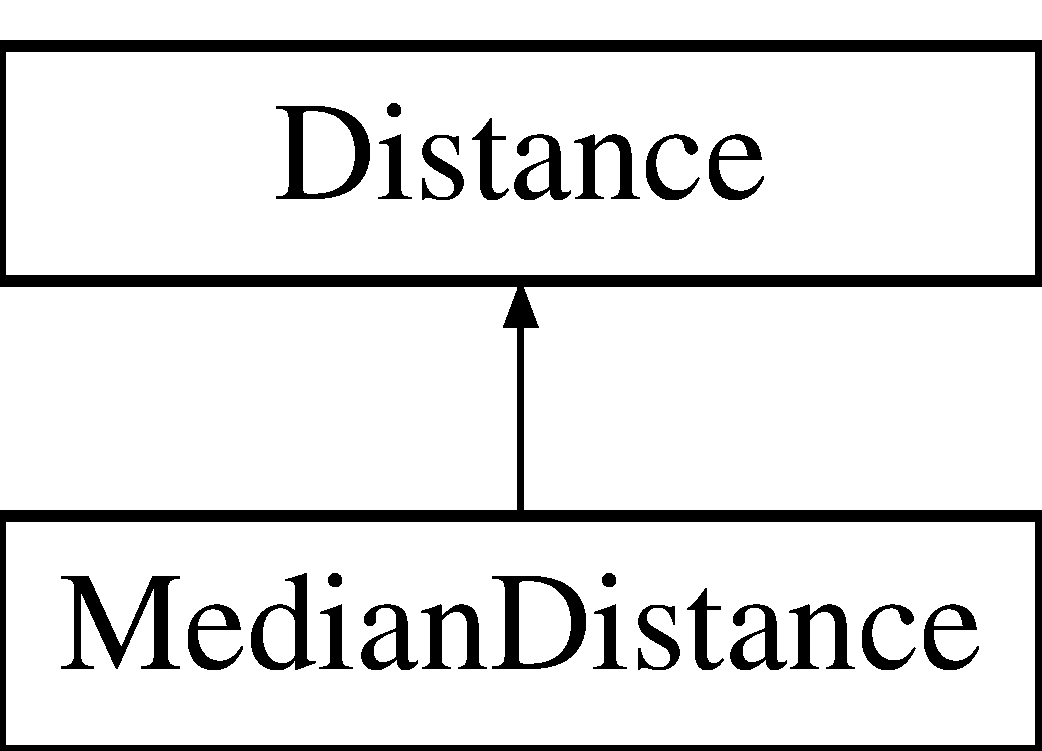
\includegraphics[height=2.000000cm]{classMedianDistance}
\end{center}
\end{figure}
\subsection*{Public Member Functions}
\begin{DoxyCompactItemize}
\item 
\hypertarget{classMedianDistance_a0b249958c04e6b9a35ffc31293fffb62}{}virtual double {\bfseries pose\+Distance} (const \hyperlink{classPose}{Pose} \&a, const \hyperlink{classPose}{Pose} \&b)\label{classMedianDistance_a0b249958c04e6b9a35ffc31293fffb62}

\end{DoxyCompactItemize}
\subsection*{Additional Inherited Members}


The documentation for this class was generated from the following files\+:\begin{DoxyCompactItemize}
\item 
Distance.\+h\item 
Distance.\+cpp\end{DoxyCompactItemize}

\hypertarget{classPoint3D}{}\section{Point3\+D Class Reference}
\label{classPoint3D}\index{Point3\+D@{Point3\+D}}


Real-\/valued points in 3 space, i.\+e. (x, y, z)  




{\ttfamily \#include $<$Point3\+D.\+h$>$}

\subsection*{Public Member Functions}
\begin{DoxyCompactItemize}
\item 
\hypertarget{classPoint3D_af4ed168ed883ea404ed363c79408e830}{}\hyperlink{classPoint3D_af4ed168ed883ea404ed363c79408e830}{Point3\+D} (double \hyperlink{classPoint3D_abf9d1f564d599503cdb114934c7044b7}{x}=0.\+0, double \hyperlink{classPoint3D_abcb44b06e310b076fa9d65dec8541dd4}{y}=0.\+0, double \hyperlink{classPoint3D_a9f4a32e3afccb3c9fe9b5cd88e179c3d}{z}=0.\+0)\label{classPoint3D_af4ed168ed883ea404ed363c79408e830}

\begin{DoxyCompactList}\small\item\em Constructor with up to 3 coordinate arguments. All arguments default to 0. \end{DoxyCompactList}\item 
\hypertarget{classPoint3D_ab637223cff9a13531cb82bea70fdf2be}{}double \hyperlink{classPoint3D_ab637223cff9a13531cb82bea70fdf2be}{X} () const \label{classPoint3D_ab637223cff9a13531cb82bea70fdf2be}

\begin{DoxyCompactList}\small\item\em Return the X coordinate of the point. \end{DoxyCompactList}\item 
\hypertarget{classPoint3D_a0321eefbe2d003c6e5de81557a938711}{}double \hyperlink{classPoint3D_a0321eefbe2d003c6e5de81557a938711}{Y} () const \label{classPoint3D_a0321eefbe2d003c6e5de81557a938711}

\begin{DoxyCompactList}\small\item\em Return the Y coordinate of the point. \end{DoxyCompactList}\item 
\hypertarget{classPoint3D_a9de6ff7d82e55b70d3c59c24cf54f2d2}{}double \hyperlink{classPoint3D_a9de6ff7d82e55b70d3c59c24cf54f2d2}{Z} () const \label{classPoint3D_a9de6ff7d82e55b70d3c59c24cf54f2d2}

\begin{DoxyCompactList}\small\item\em Return the Z coordindate of the point. \end{DoxyCompactList}\item 
\hypertarget{classPoint3D_a086f97e26ab835eb325c3e8f9200b081}{}void \hyperlink{classPoint3D_a086f97e26ab835eb325c3e8f9200b081}{set\+X} (double new\+X)\label{classPoint3D_a086f97e26ab835eb325c3e8f9200b081}

\begin{DoxyCompactList}\small\item\em Return the X coordinate of the point. \end{DoxyCompactList}\item 
\hypertarget{classPoint3D_ae14e9585590cd4454ce55e5abe1282b7}{}void \hyperlink{classPoint3D_ae14e9585590cd4454ce55e5abe1282b7}{set\+Y} (double new\+Y)\label{classPoint3D_ae14e9585590cd4454ce55e5abe1282b7}

\begin{DoxyCompactList}\small\item\em Return the Y coordinate of the point. \end{DoxyCompactList}\item 
\hypertarget{classPoint3D_af32f89789f8fc1915631a06438aa88b2}{}void \hyperlink{classPoint3D_af32f89789f8fc1915631a06438aa88b2}{set\+Z} (double new\+Z)\label{classPoint3D_af32f89789f8fc1915631a06438aa88b2}

\begin{DoxyCompactList}\small\item\em Return the Z coordindate of the point. \end{DoxyCompactList}\item 
\hypertarget{classPoint3D_afdf3bb8a874123cc5df2949204874b09}{}void \hyperlink{classPoint3D_afdf3bb8a874123cc5df2949204874b09}{scale} (double scale)\label{classPoint3D_afdf3bb8a874123cc5df2949204874b09}

\begin{DoxyCompactList}\small\item\em Vector scale the point by some scalar. \end{DoxyCompactList}\item 
\hypertarget{classPoint3D_aab49db30fa70a0f53075450d80dbfb54}{}void {\bfseries transform} (double x\+Transform, double y\+Transform, double z\+Transform)\label{classPoint3D_aab49db30fa70a0f53075450d80dbfb54}

\item 
\hypertarget{classPoint3D_a76feca0cf0787685bfc4ffdaea1340fd}{}double {\bfseries point\+Compare} (const \hyperlink{classPoint3D}{Point3\+D} p) const \label{classPoint3D_a76feca0cf0787685bfc4ffdaea1340fd}

\end{DoxyCompactItemize}
\subsection*{Protected Attributes}
\begin{DoxyCompactItemize}
\item 
\hypertarget{classPoint3D_abf9d1f564d599503cdb114934c7044b7}{}double \hyperlink{classPoint3D_abf9d1f564d599503cdb114934c7044b7}{x}\label{classPoint3D_abf9d1f564d599503cdb114934c7044b7}

\begin{DoxyCompactList}\small\item\em x coordinate (real value) \end{DoxyCompactList}\item 
\hypertarget{classPoint3D_abcb44b06e310b076fa9d65dec8541dd4}{}double \hyperlink{classPoint3D_abcb44b06e310b076fa9d65dec8541dd4}{y}\label{classPoint3D_abcb44b06e310b076fa9d65dec8541dd4}

\begin{DoxyCompactList}\small\item\em y coordinate (real value) \end{DoxyCompactList}\item 
\hypertarget{classPoint3D_a9f4a32e3afccb3c9fe9b5cd88e179c3d}{}double \hyperlink{classPoint3D_a9f4a32e3afccb3c9fe9b5cd88e179c3d}{z}\label{classPoint3D_a9f4a32e3afccb3c9fe9b5cd88e179c3d}

\begin{DoxyCompactList}\small\item\em z coordinate (real value) \end{DoxyCompactList}\end{DoxyCompactItemize}


\subsection{Detailed Description}
Real-\/valued points in 3 space, i.\+e. (x, y, z) 

\hyperlink{classPoint3D}{Point3\+D} is the base class for storing points in 3 space and accessing their coordinates. The \hyperlink{classPoseDisplay}{Pose\+Display} class will write out and display vectors of 25 Point3\+Ds (obviously, their order matters!).

The \hyperlink{classPoint3D}{Point3\+D} class as implemented here is sufficient for Programming Assignment \#1. As the semester progresses, however, students are encouraged to extend this class by adding new methods, new overloaded operators, and new data fields as necessary. As long as the \hyperlink{classPoint3D_ab637223cff9a13531cb82bea70fdf2be}{X()}, \hyperlink{classPoint3D_a0321eefbe2d003c6e5de81557a938711}{Y()}, \hyperlink{classPoint3D_a9de6ff7d82e55b70d3c59c24cf54f2d2}{Z()} methods and the $<$$<$ operator below are retained, the \hyperlink{classPoseDisplay}{Pose\+Display} class will work with modifications of the Pose3\+D class. Students are also encouraged new classes, including classes that might contain \hyperlink{classPoint3D}{Point3\+D} fields. 

The documentation for this class was generated from the following files\+:\begin{DoxyCompactItemize}
\item 
\hyperlink{Point3D_8h}{Point3\+D.\+h}\item 
Point3\+D.\+cpp\end{DoxyCompactItemize}

\hypertarget{classPose}{}\section{Pose Class Reference}
\label{classPose}\index{Pose@{Pose}}
\subsection*{Public Member Functions}
\begin{DoxyCompactItemize}
\item 
\hypertarget{classPose_a7435f9e29f346c489c830b6eeece4562}{}int {\bfseries read\+Pose} (string line)\label{classPose_a7435f9e29f346c489c830b6eeece4562}

\item 
\hypertarget{classPose_ac044bc60b60d7ad3b8fa1db02b6b0b07}{}int {\bfseries write\+Pose} (\hyperlink{classPoseDisplay}{Pose\+Display} \&p\+Display)\label{classPose_ac044bc60b60d7ad3b8fa1db02b6b0b07}

\item 
\hypertarget{classPose_a6db9c0f53878ebd46e721c81f138d32d}{}double {\bfseries pose\+Compare} (\hyperlink{classPose}{Pose} p)\label{classPose_a6db9c0f53878ebd46e721c81f138d32d}

\item 
\hypertarget{classPose_a8252053c77047d1e2d2e79d393e3adef}{}\hyperlink{classPoint3D}{Point3\+D} \& {\bfseries get\+Point3\+D} (int position)\label{classPose_a8252053c77047d1e2d2e79d393e3adef}

\item 
\hypertarget{classPose_a06f956b0ab2b046cb2385f10ac79ebc1}{}const \hyperlink{classPoint3D}{Point3\+D} \& {\bfseries get\+Point3\+D} (int position) const \label{classPose_a06f956b0ab2b046cb2385f10ac79ebc1}

\end{DoxyCompactItemize}
\subsection*{Protected Attributes}
\begin{DoxyCompactItemize}
\item 
\hypertarget{classPose_ab9f5423ef45012b900d1f968d89e2154}{}vector$<$ \hyperlink{classPoint3D}{Point3\+D} $>$ {\bfseries points}\label{classPose_ab9f5423ef45012b900d1f968d89e2154}

\end{DoxyCompactItemize}


The documentation for this class was generated from the following files\+:\begin{DoxyCompactItemize}
\item 
Pose.\+h\item 
Pose.\+cpp\end{DoxyCompactItemize}

\hypertarget{classPoseDisplay}{}\section{Pose\+Display Class Reference}
\label{classPoseDisplay}\index{Pose\+Display@{Pose\+Display}}


Class for outputting and (optionally) displaying body poses expressed as a vector of 25 Point3\+Ds.  




{\ttfamily \#include $<$Pose\+Display.\+h$>$}

\subsection*{Public Member Functions}
\begin{DoxyCompactItemize}
\item 
\hyperlink{classPoseDisplay_aa1b69b1d84ef195caccbc763d1028c60}{Pose\+Display} (const string \&output\+\_\+filename, bool visual\+\_\+display=true)
\begin{DoxyCompactList}\small\item\em Constructor. May throw a std\+::exception if the window or file can\textquotesingle{}t be opened. \end{DoxyCompactList}\item 
\hypertarget{classPoseDisplay_abe76af64858d725b705855056facbf3f}{}\hyperlink{classPoseDisplay_abe76af64858d725b705855056facbf3f}{$\sim$\+Pose\+Display} ()\label{classPoseDisplay_abe76af64858d725b705855056facbf3f}

\begin{DoxyCompactList}\small\item\em Destructor. Closes the X11 window (if its open) and the output file. \end{DoxyCompactList}\item 
\hypertarget{classPoseDisplay_a40edcdb672d0f785c4966021d6a2c9e2}{}bool \hyperlink{classPoseDisplay_a40edcdb672d0f785c4966021d6a2c9e2}{Pose} (const vector$<$ \hyperlink{classPoint3D}{Point3\+D} $>$ \&data, int ms\+\_\+delay=33)\label{classPoseDisplay_a40edcdb672d0f785c4966021d6a2c9e2}

\begin{DoxyCompactList}\small\item\em Write a pose (25 body points) to the output file, and (optionally) display it to the window. ms\+\_\+delay is the delay for viewing in milliseconds. \end{DoxyCompactList}\item 
\hypertarget{classPoseDisplay_a7dfe55ebb0ea62ba9f6852e2e61ec3d3}{}void \hyperlink{classPoseDisplay_a7dfe55ebb0ea62ba9f6852e2e61ec3d3}{Pause} (int delay=33)\label{classPoseDisplay_a7dfe55ebb0ea62ba9f6852e2e61ec3d3}

\begin{DoxyCompactList}\small\item\em Pause briefly, to allow display to be seen. Units of pause are millisecond, so 33 is roughly frame rate. \end{DoxyCompactList}\end{DoxyCompactItemize}
\subsection*{Protected Member Functions}
\begin{DoxyCompactItemize}
\item 
\hypertarget{classPoseDisplay_af9f9376866ce200739343b6ea5a9f2f4}{}bool \hyperlink{classPoseDisplay_af9f9376866ce200739343b6ea5a9f2f4}{Write\+Pose} (const vector$<$ \hyperlink{classPoint3D}{Point3\+D} $>$ \&data)\label{classPoseDisplay_af9f9376866ce200739343b6ea5a9f2f4}

\begin{DoxyCompactList}\small\item\em Write a pose (25 body points) to the output file. \end{DoxyCompactList}\item 
\hypertarget{classPoseDisplay_af54050c57f676a23c6b5bdabdd0947db}{}void \hyperlink{classPoseDisplay_af54050c57f676a23c6b5bdabdd0947db}{Draw\+Pose} (const vector$<$ \hyperlink{classPoint3D}{Point3\+D} $>$ \&data) const \label{classPoseDisplay_af54050c57f676a23c6b5bdabdd0947db}

\begin{DoxyCompactList}\small\item\em Draw a pose (25 body points) to the X11 window. \end{DoxyCompactList}\item 
\hypertarget{classPoseDisplay_aca5c1b0509ca136e5de383cbc9d7a1eb}{}void \hyperlink{classPoseDisplay_aca5c1b0509ca136e5de383cbc9d7a1eb}{Draw\+Connection} (const \hyperlink{classPoint3D}{Point3\+D} \&pt1, const \hyperlink{classPoint3D}{Point3\+D} \&pt2) const \label{classPoseDisplay_aca5c1b0509ca136e5de383cbc9d7a1eb}

\begin{DoxyCompactList}\small\item\em Draw a line connecting two body points in all three views. \end{DoxyCompactList}\item 
\hypertarget{classPoseDisplay_af7cab412d8dab3ea4f5482a27fe2dcab}{}bool \hyperlink{classPoseDisplay_af7cab412d8dab3ea4f5482a27fe2dcab}{Open\+Output\+File} ()\label{classPoseDisplay_af7cab412d8dab3ea4f5482a27fe2dcab}

\begin{DoxyCompactList}\small\item\em Open the output file. Return false if unable to open file. \end{DoxyCompactList}\item 
bool \hyperlink{classPoseDisplay_a544a1d80438850ccfcc45107706de6cd}{Open\+Output\+Window} ()
\begin{DoxyCompactList}\small\item\em Open an X11 window. Return false if unable to do so. \end{DoxyCompactList}\item 
\hypertarget{classPoseDisplay_a0a2636aa2f67254c5de8f18c46660aeb}{}void \hyperlink{classPoseDisplay_a0a2636aa2f67254c5de8f18c46660aeb}{Draw\+Window\+Frames} () const \label{classPoseDisplay_a0a2636aa2f67254c5de8f18c46660aeb}

\begin{DoxyCompactList}\small\item\em Draw the borders, axes and labels associated with all three views to the X11 window. \end{DoxyCompactList}\item 
\hypertarget{classPoseDisplay_af6c16081d868902bbbc34d8640d185e3}{}void \hyperlink{classPoseDisplay_af6c16081d868902bbbc34d8640d185e3}{Draw\+View} (string label, string horizontal\+\_\+axis, string vertical\+\_\+axis, int frame\+\_\+number) const \label{classPoseDisplay_af6c16081d868902bbbc34d8640d185e3}

\begin{DoxyCompactList}\small\item\em Draw the axes and labels associated with one view to the X11 window. \end{DoxyCompactList}\item 
\hypertarget{classPoseDisplay_a9708b913ab7a6258e5a67e6fe79a23a4}{}void \hyperlink{classPoseDisplay_a9708b913ab7a6258e5a67e6fe79a23a4}{Draw\+View\+Line} (int view\+\_\+number, double x1, double y1, double x2, double y2) const \label{classPoseDisplay_a9708b913ab7a6258e5a67e6fe79a23a4}

\begin{DoxyCompactList}\small\item\em Draw a single line to a single image view. \end{DoxyCompactList}\item 
\hypertarget{classPoseDisplay_a5c2541bf1dc46748a80fc4e8bac2736a}{}void \hyperlink{classPoseDisplay_a5c2541bf1dc46748a80fc4e8bac2736a}{Initialize\+Skeleton} ()\label{classPoseDisplay_a5c2541bf1dc46748a80fc4e8bac2736a}

\begin{DoxyCompactList}\small\item\em Initialize the vector of pairs that signals which body parts connect to which other body parts. \end{DoxyCompactList}\end{DoxyCompactItemize}
\subsection*{Protected Attributes}
\begin{DoxyCompactItemize}
\item 
\hypertarget{classPoseDisplay_a5d2e9d3f9caa69c8eb1c348c56ba7a51}{}bool \hyperlink{classPoseDisplay_a5d2e9d3f9caa69c8eb1c348c56ba7a51}{displayp}\label{classPoseDisplay_a5d2e9d3f9caa69c8eb1c348c56ba7a51}

\begin{DoxyCompactList}\small\item\em Whether or not poses are being displayed to a window. \end{DoxyCompactList}\item 
\hypertarget{classPoseDisplay_a9a903a2b1a3d4985bfb36da23e5ae0fc}{}Display $\ast$ \hyperlink{classPoseDisplay_a9a903a2b1a3d4985bfb36da23e5ae0fc}{display\+\_\+ptr}\label{classPoseDisplay_a9a903a2b1a3d4985bfb36da23e5ae0fc}

\begin{DoxyCompactList}\small\item\em Pointer to the X11 display structure. \end{DoxyCompactList}\item 
\hypertarget{classPoseDisplay_a46c88e5385d36c96018000c22178734d}{}Window \hyperlink{classPoseDisplay_a46c88e5385d36c96018000c22178734d}{window}\label{classPoseDisplay_a46c88e5385d36c96018000c22178734d}

\begin{DoxyCompactList}\small\item\em X11 window structure (one application can have many windows) \end{DoxyCompactList}\item 
\hypertarget{classPoseDisplay_afccdac510a02e9447f54cdb896cf3c75}{}G\+C \hyperlink{classPoseDisplay_afccdac510a02e9447f54cdb896cf3c75}{graphics\+\_\+context}\label{classPoseDisplay_afccdac510a02e9447f54cdb896cf3c75}

\begin{DoxyCompactList}\small\item\em X11 graphics context structure (holds colors, line widths, etc.) \end{DoxyCompactList}\item 
\hypertarget{classPoseDisplay_a4c736f7ac4b51817117c61daaf278937}{}string \hyperlink{classPoseDisplay_a4c736f7ac4b51817117c61daaf278937}{filename}\label{classPoseDisplay_a4c736f7ac4b51817117c61daaf278937}

\begin{DoxyCompactList}\small\item\em Filename that poses will be recorded to. \end{DoxyCompactList}\item 
\hypertarget{classPoseDisplay_aa50c8842e3aff32a56a560e0199c81a8}{}ofstream \hyperlink{classPoseDisplay_aa50c8842e3aff32a56a560e0199c81a8}{ostr}\label{classPoseDisplay_aa50c8842e3aff32a56a560e0199c81a8}

\begin{DoxyCompactList}\small\item\em Output stream associated with filename. \end{DoxyCompactList}\item 
\hypertarget{classPoseDisplay_a85f6a7c05c2c97113cb614a15b2867e4}{}vector$<$ pair$<$ int, int $>$ $>$ \hyperlink{classPoseDisplay_a85f6a7c05c2c97113cb614a15b2867e4}{connections}\label{classPoseDisplay_a85f6a7c05c2c97113cb614a15b2867e4}

\begin{DoxyCompactList}\small\item\em Point connection information. An $<$i,j$>$ pair indicates that Point i is connected to Point j. \end{DoxyCompactList}\end{DoxyCompactItemize}


\subsection{Detailed Description}
Class for outputting and (optionally) displaying body poses expressed as a vector of 25 Point3\+Ds. 

The \hyperlink{classPoseDisplay}{Pose\+Display} class has two purposes. The first is to display body poses to the screen so that you can see them. The second is to record all the displayed poses to a file, as a record of what your program displayed that we can grade.

The public interface to \hyperlink{classPoseDisplay}{Pose\+Display} is simple. It has a constructor, a destructor, and a single public method called \hyperlink{classPose}{Pose}. The constructor takes a file name as an argument. This is the file it will write the poses to. There is an optional second argument called visual\+\_\+display that defaults to true. When this argument is true, poses will be drawn to the screen. When it is false, poses are written to the file but never displayed; in fact, no X11 window is ever created. This will be useful later in the semester when some assignments are graded by efficiency. The \hyperlink{classPose}{Pose} method takes a body pose, i.\+e. a vector of 25 Point3\+Ds, writes it to the output file, and displays it to the screen if visual\+\_\+display is true. The destructor simply cleans up when a \hyperlink{classPoseDisplay}{Pose\+Display} is deleted or falls out of scope by destroying the window (if applicable) and closing the output file. 

\subsection{Constructor \& Destructor Documentation}
\hypertarget{classPoseDisplay_aa1b69b1d84ef195caccbc763d1028c60}{}\index{Pose\+Display@{Pose\+Display}!Pose\+Display@{Pose\+Display}}
\index{Pose\+Display@{Pose\+Display}!Pose\+Display@{Pose\+Display}}
\subsubsection[{Pose\+Display(const string \&output\+\_\+filename, bool visual\+\_\+display=true)}]{\setlength{\rightskip}{0pt plus 5cm}Pose\+Display\+::\+Pose\+Display (
\begin{DoxyParamCaption}
\item[{const string \&}]{output\+\_\+filename, }
\item[{bool}]{visual\+\_\+display = {\ttfamily true}}
\end{DoxyParamCaption}
)}\label{classPoseDisplay_aa1b69b1d84ef195caccbc763d1028c60}


Constructor. May throw a std\+::exception if the window or file can\textquotesingle{}t be opened. 


\begin{DoxyParams}{Parameters}
{\em output\+\_\+filename} & is the name of the file that will be opened for output, so that all poses will be saved to this file. \\
\hline
{\em visual\+\_\+display} & determines whether or not poses are displayed to an X11 window (and whether an X11 window is ever created).\\
\hline
\end{DoxyParams}
This constructor will throw a std\+::exception() if it is unable to open the output file, or if visual\+\_\+display is true but it is unable to open an X11 window. 

\subsection{Member Function Documentation}
\hypertarget{classPoseDisplay_a544a1d80438850ccfcc45107706de6cd}{}\index{Pose\+Display@{Pose\+Display}!Open\+Output\+Window@{Open\+Output\+Window}}
\index{Open\+Output\+Window@{Open\+Output\+Window}!Pose\+Display@{Pose\+Display}}
\subsubsection[{Open\+Output\+Window()}]{\setlength{\rightskip}{0pt plus 5cm}bool Pose\+Display\+::\+Open\+Output\+Window (
\begin{DoxyParamCaption}
{}
\end{DoxyParamCaption}
)\hspace{0.3cm}{\ttfamily [protected]}}\label{classPoseDisplay_a544a1d80438850ccfcc45107706de6cd}


Open an X11 window. Return false if unable to do so. 

This method relies on the X11 library to crate the display window. If X\+Open\+Display, X\+Create\+Window or X\+Create\+C\+G return N\+U\+L\+L (in their attempt to create a display, window and graphics context, respectively), this method will return false. Otherwise it returns true. The window created will be empty (cleared); the headers and boundary are drawn when poses are displayed. 

The documentation for this class was generated from the following files\+:\begin{DoxyCompactItemize}
\item 
\hyperlink{PoseDisplay_8h}{Pose\+Display.\+h}\item 
\hyperlink{PoseDisplay_8cpp}{Pose\+Display.\+cpp}\end{DoxyCompactItemize}

\hypertarget{classPoseSequence}{}\section{Pose\+Sequence Class Reference}
\label{classPoseSequence}\index{Pose\+Sequence@{Pose\+Sequence}}
\subsection*{Public Member Functions}
\begin{DoxyCompactItemize}
\item 
\hypertarget{classPoseSequence_a86f364410d68c0fbdb44671702d691ef}{}int {\bfseries read\+From\+Name} (const char $\ast$file\+Name)\label{classPoseSequence_a86f364410d68c0fbdb44671702d691ef}

\item 
\hypertarget{classPoseSequence_a9c572d095fd38ab1eb5a366c5a5a849f}{}int {\bfseries read\+Pose\+Sequence} (fstream \&file)\label{classPoseSequence_a9c572d095fd38ab1eb5a366c5a5a849f}

\item 
\hypertarget{classPoseSequence_a9cea0db6a913505e585ffa8c9667b913}{}int {\bfseries write\+Pose\+Sequence} (\hyperlink{classPoseDisplay}{Pose\+Display} \&p\+Display)\label{classPoseSequence_a9cea0db6a913505e585ffa8c9667b913}

\item 
\hypertarget{classPoseSequence_af425c0eec2de254d105feac4efaa033b}{}double {\bfseries pose\+Sequence\+Compare} (ostream \&file, \hyperlink{classPoseSequence}{Pose\+Sequence} \&other)\label{classPoseSequence_af425c0eec2de254d105feac4efaa033b}

\item 
\hypertarget{classPoseSequence_a50daa04df4f17a1741bf689fee73561c}{}int {\bfseries size} () const \label{classPoseSequence_a50daa04df4f17a1741bf689fee73561c}

\item 
\hypertarget{classPoseSequence_a6ac72caee4b7602f3d508434963e963d}{}\hyperlink{classPose}{Pose} {\bfseries get\+Pose} (int i) const \label{classPoseSequence_a6ac72caee4b7602f3d508434963e963d}

\end{DoxyCompactItemize}
\subsection*{Protected Attributes}
\begin{DoxyCompactItemize}
\item 
\hypertarget{classPoseSequence_a0717d1235bac6edfee8b70b425fcbf98}{}vector$<$ \hyperlink{classPose}{Pose} $>$ {\bfseries poses}\label{classPoseSequence_a0717d1235bac6edfee8b70b425fcbf98}

\end{DoxyCompactItemize}


The documentation for this class was generated from the following files\+:\begin{DoxyCompactItemize}
\item 
Pose\+Sequence.\+h\item 
Pose\+Sequence.\+cpp\end{DoxyCompactItemize}

\chapter{File Documentation}
\hypertarget{Point3D_8h}{}\section{Point3\+D.\+h File Reference}
\label{Point3D_8h}\index{Point3\+D.\+h@{Point3\+D.\+h}}


Contains the \hyperlink{classPoint3D}{Point3\+D} class declaration (header)  


{\ttfamily \#include $<$iostream$>$}\\*
{\ttfamily \#include $<$cmath$>$}\\*
\subsection*{Classes}
\begin{DoxyCompactItemize}
\item 
class \hyperlink{classPoint3D}{Point3\+D}
\begin{DoxyCompactList}\small\item\em Real-\/valued points in 3 space, i.\+e. (x, y, z) \end{DoxyCompactList}\end{DoxyCompactItemize}
\subsection*{Functions}
\begin{DoxyCompactItemize}
\item 
\hypertarget{Point3D_8h_a71c7ddf0ed38d20b0541707e9f7d4fbb}{}ostream \& \hyperlink{Point3D_8h_a71c7ddf0ed38d20b0541707e9f7d4fbb}{operator$<$$<$} (ostream \&ostr, const \hyperlink{classPoint3D}{Point3\+D} \&pt)\label{Point3D_8h_a71c7ddf0ed38d20b0541707e9f7d4fbb}

\begin{DoxyCompactList}\small\item\em Overload of $<$$<$ operator for \hyperlink{classPoint3D}{Point3\+D}. Prints out as three real values, separated by spaces with a trailing space. \end{DoxyCompactList}\end{DoxyCompactItemize}


\subsection{Detailed Description}
Contains the \hyperlink{classPoint3D}{Point3\+D} class declaration (header) 

Unless/until extended by students, there is no Point3\+D.\+cpp file, as all the methods of \hyperlink{classPoint3D}{Point3\+D} are inline. 
\hypertarget{PoseDisplay_8cpp}{}\section{Pose\+Display.\+cpp File Reference}
\label{PoseDisplay_8cpp}\index{Pose\+Display.\+cpp@{Pose\+Display.\+cpp}}


Contains the \hyperlink{classPoseDisplay}{Pose\+Display} class implementation.  


{\ttfamily \#include $<$Pose\+Display.\+h$>$}\\*
{\ttfamily \#include $<$exception$>$}\\*
{\ttfamily \#include $<$iostream$>$}\\*
{\ttfamily \#include $<$math.\+h$>$}\\*
\subsection*{Functions}
\begin{DoxyCompactItemize}
\item 
\hypertarget{PoseDisplay_8cpp_a03e3598ee22d7efcd268acf1d1ca75d0}{}int \hyperlink{PoseDisplay_8cpp_a03e3598ee22d7efcd268acf1d1ca75d0}{Handle\+X11\+Errors} (Display $\ast$d, X\+Error\+Event $\ast$e)\label{PoseDisplay_8cpp_a03e3598ee22d7efcd268acf1d1ca75d0}

\begin{DoxyCompactList}\small\item\em X11 Error Handler. Make X11 throw std\+::exception(), so that all errors can be handled the same way. \end{DoxyCompactList}\end{DoxyCompactItemize}
\subsection*{Variables}
\begin{DoxyCompactItemize}
\item 
\hypertarget{PoseDisplay_8cpp_a02b852ef5173bab9e7422e75c6160a05}{}const int \hyperlink{PoseDisplay_8cpp_a02b852ef5173bab9e7422e75c6160a05}{Header\+Height} = 20\label{PoseDisplay_8cpp_a02b852ef5173bab9e7422e75c6160a05}

\begin{DoxyCompactList}\small\item\em Height of header used to label view planes (e.\+g. \char`\"{}\+X\+Y Plane\char`\"{}) \end{DoxyCompactList}\item 
\hypertarget{PoseDisplay_8cpp_a72533e710da237a19df290ab5bc33c67}{}const int \hyperlink{PoseDisplay_8cpp_a72533e710da237a19df290ab5bc33c67}{Frame\+Size} = 240\label{PoseDisplay_8cpp_a72533e710da237a19df290ab5bc33c67}

\begin{DoxyCompactList}\small\item\em Size of (square) frame that contains both the pose view and the labeled axes. \end{DoxyCompactList}\item 
\hypertarget{PoseDisplay_8cpp_a88964f5ce40bf4f0054457fc6c416e6b}{}const int \hyperlink{PoseDisplay_8cpp_a88964f5ce40bf4f0054457fc6c416e6b}{View\+Size} = 200\label{PoseDisplay_8cpp_a88964f5ce40bf4f0054457fc6c416e6b}

\begin{DoxyCompactList}\small\item\em Height of (square) pose view containing the skeleton figure representing a pose. \end{DoxyCompactList}\item 
\hypertarget{PoseDisplay_8cpp_a2f9637b12bcd6f9452233804b1373fc6}{}const int \hyperlink{PoseDisplay_8cpp_a2f9637b12bcd6f9452233804b1373fc6}{View\+Offset} = (\hyperlink{PoseDisplay_8cpp_a72533e710da237a19df290ab5bc33c67}{Frame\+Size} -\/ \hyperlink{PoseDisplay_8cpp_a88964f5ce40bf4f0054457fc6c416e6b}{View\+Size}) / 2\label{PoseDisplay_8cpp_a2f9637b12bcd6f9452233804b1373fc6}

\begin{DoxyCompactList}\small\item\em \hyperlink{classDistance}{Distance} from the beginning of the frame to the beginning of the view. \end{DoxyCompactList}\item 
\hypertarget{PoseDisplay_8cpp_a00c2e195d5351bdc92a84a7fc4c5a7c7}{}const int \hyperlink{PoseDisplay_8cpp_a00c2e195d5351bdc92a84a7fc4c5a7c7}{Window\+Height} = \hyperlink{PoseDisplay_8cpp_a72533e710da237a19df290ab5bc33c67}{Frame\+Size} + \hyperlink{PoseDisplay_8cpp_a02b852ef5173bab9e7422e75c6160a05}{Header\+Height}\label{PoseDisplay_8cpp_a00c2e195d5351bdc92a84a7fc4c5a7c7}

\begin{DoxyCompactList}\small\item\em Total height of the X11 window (frame + header) \end{DoxyCompactList}\item 
\hypertarget{PoseDisplay_8cpp_a22d61ce60159be2579f9b403d2d6b72a}{}const int \hyperlink{PoseDisplay_8cpp_a22d61ce60159be2579f9b403d2d6b72a}{Window\+Width} = 3 $\ast$ \hyperlink{PoseDisplay_8cpp_a72533e710da237a19df290ab5bc33c67}{Frame\+Size}\label{PoseDisplay_8cpp_a22d61ce60159be2579f9b403d2d6b72a}

\begin{DoxyCompactList}\small\item\em Total width of the X11 window (holds three frames sides by side) \end{DoxyCompactList}\item 
\hypertarget{PoseDisplay_8cpp_a8efa8034bc39024e2d18e80ab808eb10}{}const int \hyperlink{PoseDisplay_8cpp_a8efa8034bc39024e2d18e80ab808eb10}{View\+Top} = \hyperlink{PoseDisplay_8cpp_a02b852ef5173bab9e7422e75c6160a05}{Header\+Height} + \hyperlink{PoseDisplay_8cpp_a2f9637b12bcd6f9452233804b1373fc6}{View\+Offset}\label{PoseDisplay_8cpp_a8efa8034bc39024e2d18e80ab808eb10}

\begin{DoxyCompactList}\small\item\em Y coordinate of the top of a view (all three views are at the same height) \end{DoxyCompactList}\item 
\hypertarget{PoseDisplay_8cpp_a467d38a411c515bb537f71d9c7a1c352}{}const int \hyperlink{PoseDisplay_8cpp_a467d38a411c515bb537f71d9c7a1c352}{View\+Middle} = \hyperlink{PoseDisplay_8cpp_a8efa8034bc39024e2d18e80ab808eb10}{View\+Top} + (\hyperlink{PoseDisplay_8cpp_a88964f5ce40bf4f0054457fc6c416e6b}{View\+Size} / 2)\label{PoseDisplay_8cpp_a467d38a411c515bb537f71d9c7a1c352}

\begin{DoxyCompactList}\small\item\em Y coordinate of the middle of a view (all three views are at the same height) \end{DoxyCompactList}\item 
\hypertarget{PoseDisplay_8cpp_a4b203c089a299104be5ccfe00854c600}{}const int \hyperlink{PoseDisplay_8cpp_a4b203c089a299104be5ccfe00854c600}{View\+Bottom} = \hyperlink{PoseDisplay_8cpp_a8efa8034bc39024e2d18e80ab808eb10}{View\+Top} + \hyperlink{PoseDisplay_8cpp_a88964f5ce40bf4f0054457fc6c416e6b}{View\+Size}\label{PoseDisplay_8cpp_a4b203c089a299104be5ccfe00854c600}

\begin{DoxyCompactList}\small\item\em Y coordinate of the bottom of a view (all three views are at the same height) \end{DoxyCompactList}\item 
\hypertarget{PoseDisplay_8cpp_a1c693a1232d2a944f343c63f8e54c4f2}{}const double \hyperlink{PoseDisplay_8cpp_a1c693a1232d2a944f343c63f8e54c4f2}{View\+Scale} = \hyperlink{PoseDisplay_8cpp_a88964f5ce40bf4f0054457fc6c416e6b}{View\+Size} / 2.\+0\label{PoseDisplay_8cpp_a1c693a1232d2a944f343c63f8e54c4f2}

\begin{DoxyCompactList}\small\item\em Scale factor for going from logical coordinates (-\/1 to 1) to pixels in the view. \end{DoxyCompactList}\end{DoxyCompactItemize}


\subsection{Detailed Description}
Contains the \hyperlink{classPoseDisplay}{Pose\+Display} class implementation. 

Not surprisingly, the declaration for the \hyperlink{classPoseDisplay}{Pose\+Display} class is in \hyperlink{PoseDisplay_8h}{Pose\+Display.\+h}. 
\hypertarget{PoseDisplay_8h}{}\section{Pose\+Display.\+h File Reference}
\label{PoseDisplay_8h}\index{Pose\+Display.\+h@{Pose\+Display.\+h}}


Contains the \hyperlink{classPoseDisplay}{Pose\+Display} class declaration (header)  


{\ttfamily \#include $<$Point3\+D.\+h$>$}\\*
{\ttfamily \#include $<$X11/\+Xlib.\+h$>$}\\*
{\ttfamily \#include $<$unistd.\+h$>$}\\*
{\ttfamily \#include $<$string$>$}\\*
{\ttfamily \#include $<$vector$>$}\\*
{\ttfamily \#include $<$utility$>$}\\*
{\ttfamily \#include $<$fstream$>$}\\*
{\ttfamily \#include $<$thread$>$}\\*
{\ttfamily \#include $<$chrono$>$}\\*
\subsection*{Classes}
\begin{DoxyCompactItemize}
\item 
class \hyperlink{classPoseDisplay}{Pose\+Display}
\begin{DoxyCompactList}\small\item\em Class for outputting and (optionally) displaying body poses expressed as a vector of 25 Point3\+Ds. \end{DoxyCompactList}\end{DoxyCompactItemize}


\subsection{Detailed Description}
Contains the \hyperlink{classPoseDisplay}{Pose\+Display} class declaration (header) 

Not surprisingly, the implementation for the \hyperlink{classPoseDisplay}{Pose\+Display} class is in \hyperlink{PoseDisplay_8cpp}{Pose\+Display.\+cpp}. This file depends on the X11 graphics library. 
%--- End generated contents ---

% Index
\backmatter
\newpage
\phantomsection
\clearemptydoublepage
\addcontentsline{toc}{chapter}{Index}
\printindex

\end{document}
